\documentclass[border=5pt]{standalone}
\usepackage{tikz}
\usepackage{tikz-3dplot}
\usetikzlibrary{arrows.meta, 3d, perspective, calc}
\usepackage{amsmath}
\begin{document}
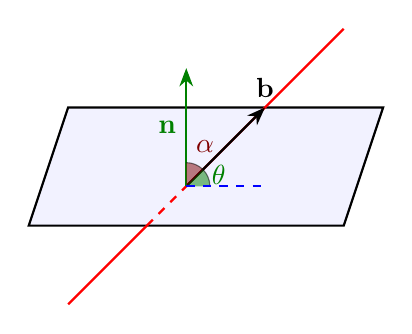
\begin{tikzpicture}[>=Stealth]
    % Plane
    \fill[blue!10, opacity=0.5] (0,0) -- (4,0) -- (4.5,1.5) -- (0.5,1.5) -- cycle;
    \draw[thick] (0,0) -- (4,0) -- (4.5,1.5) -- (0.5,1.5) -- cycle;

    % Line
    \draw[thick, red] (2,0.5) -- (4,2.5);
    \draw[thick, red, dashed] (1.5,0) -- (2,0.5);
    \draw[thick, red] (0.5,-1) -- (1.5,0);
    \draw[->, thick] (2,0.5) -- +(1,1) node[above] {$\mathbf{b}$};

    % Normal vector
    \draw[->, thick, green!50!black] (2,0.5) -- node[left] {$\mathbf{n}$} (2,0.75 |- 0,2);

    % Angle

    \begin{scope}
        \path[clip] (2,0.5) -- (3,1.5) -- (3,0.5);
        \fill[green!50!black, opacity=0.5, draw=black] (2,0.5) circle (3mm);
        \end{scope}
    \node[right, green!50!black] at (2.2,0.65) {$\theta$};

    \begin{scope}
        \path[clip] (2,0.5) -- (3,1.5) -- (2,1.5);
        \fill[red!50!black, opacity=0.5, draw=black] (2,0.5) circle (3mm);
        \end{scope}
    \node[right, red!50!black] at (2,1) {$\alpha$};

    \draw[thick, blue, dashed] (2,0.5) -- (3,0.5);
  \end{tikzpicture}
\end{document}
